
\begin{center}
\begin{tikzpicture}[node distance=2cm]
    \node (start) [action] {Action: User transfers BTC to deposit account (ETH address)};
    \node (step1) [action, below of=start] {Action: User calls notify on BTC bridge with deposit account};
    \node (step2) [event, below of=step1] {Event: Minter notification event};
    \node (step3) [operation, below of=step2] {Operation: Wait for transfer to be confirmed};
    \node (step4) [operation, below of=step3] {Operation: Transfer CKBTC to the main canister account};
    \node (step5) [operation, below of=step4] {Operation: Create mint order and send to EVM (standard flow)};

    \draw [arrow] (start) -- (step1);
    \draw [arrow] (step1) -- (step2);
    \draw [arrow] (step2) -- (step3);
    \draw [arrow] (step3) -- (step4);
    \draw [arrow] (step4) -- (step5);
\end{tikzpicture}

\vspace{2cm}

\textbf{Withdraw Process}

\vspace{2cm}


\begin{tikzpicture}[node distance=2cm]
    \node (start) [process] {Standard flow};
    \node (step1) [event, below of=start] {Event: Burn event contains the address of where to transfer the BTC};
    \node (step2) [operation, below of=step1] {Operation: Mint Base Token (transfer order on CKBTC to burn)};

    \draw [arrow] (start) -- (step1);
    \draw [arrow] (step1) -- (step2);
\end{tikzpicture}
\end{center}

\vskip 2em;





\begin{center}
\begin{tikzpicture}[node distance=2cm]
    \node (start) [action] {Action: User transfers BTC to deposit account (ETH address)};
    \node (step1) [action, below of=start] {Action: User calls notify on BTC bridge with deposit account};
    \node (step2) [event, below of=step1] {Event: Minter notification event};
    \node (step3) [operation, below of=step2] {Operation: Wait for transfer to be confirmed};
    \node (step4) [operation, below of=step3] {Operation: Transfer CKBTC to the main canister account};
    \node (step5) [operation, below of=step4] {Operation: Create mint order and send to EVM (standard flow)};

    \draw [arrow] (start) -- (step1);
    \draw [arrow] (step1) -- (step2);
    \draw [arrow] (step2) -- (step3);
    \draw [arrow] (step3) -- (step4);
    \draw [arrow] (step4) -- (step5);
\end{tikzpicture}

\vspace{2cm}

\textbf{Withdraw Process}

\vspace{2cm}


\begin{tikzpicture}[node distance=2cm]
    \node (start) [process] {Standard flow};
    \node (step1) [event, below of=start] {Event: Burn event contains the address of where to transfer the BTC};
    \node (step2) [operation, below of=step1] {Operation: Mint Base Token (transfer order on CKBTC to burn)};

    \draw [arrow] (start) -- (step1);
    \draw [arrow] (step1) -- (step2);
\end{tikzpicture}
\end{center}

\vskip 2em;



\begin{center}
\begin{tikzpicture}[node distance=2cm]
    \node (start) [action] {Action: User transfers runes to deposit account (ETH address)};
    \node (step1) [action, below of=start] {Action: User calls notify on Rune bridge with deposit account};
    \node (step2) [event, below of=step1] {Event: Minter notification event};
    \node (step3) [operation, below of=step2] {Operation: Wait for transfer to be confirmed};
    \node (step4) [operation, below of=step3] {Operation: Get rune contents of UTXOs from indexers};
    \node (step5) [operation, below of=step4] {Operation:  Mark UTXOs as spent/minted, create mint order and send to EVM (standard flow)};

    \draw [arrow] (start) -- (step1);
    \draw [arrow] (step1) -- (step2);
    \draw [arrow] (step2) -- (step3);
    \draw [arrow] (step3) -- (step4);
    \draw [arrow] (step4) -- (step5);
\end{tikzpicture}

\vspace{1cm}

\textbf{Withdraw Process}
\vspace{1cm}

\begin{tikzpicture}[node distance=2cm]
    \node (start) [action] {Action: User transfers fee BTC to deposit account (ETH address)};
    \node (step1) [process, below of=start] {Standard flow};
    \node (step2) [event, below of=step1] {Event: Burn event contains the address of where to transfer the BTC};
    \node (step3) [operation, below of=step2] {Operation: Mint Base Token (create and send BTC transaction)};

    \draw [arrow] (start) -- (step1);
    \draw [arrow] (step1) -- (step2);
    \draw [arrow] (step2) -- (step3);
\end{tikzpicture}
\end{center}


\subsection{ICRC}

    \begin{figure}[H]
        \centering
        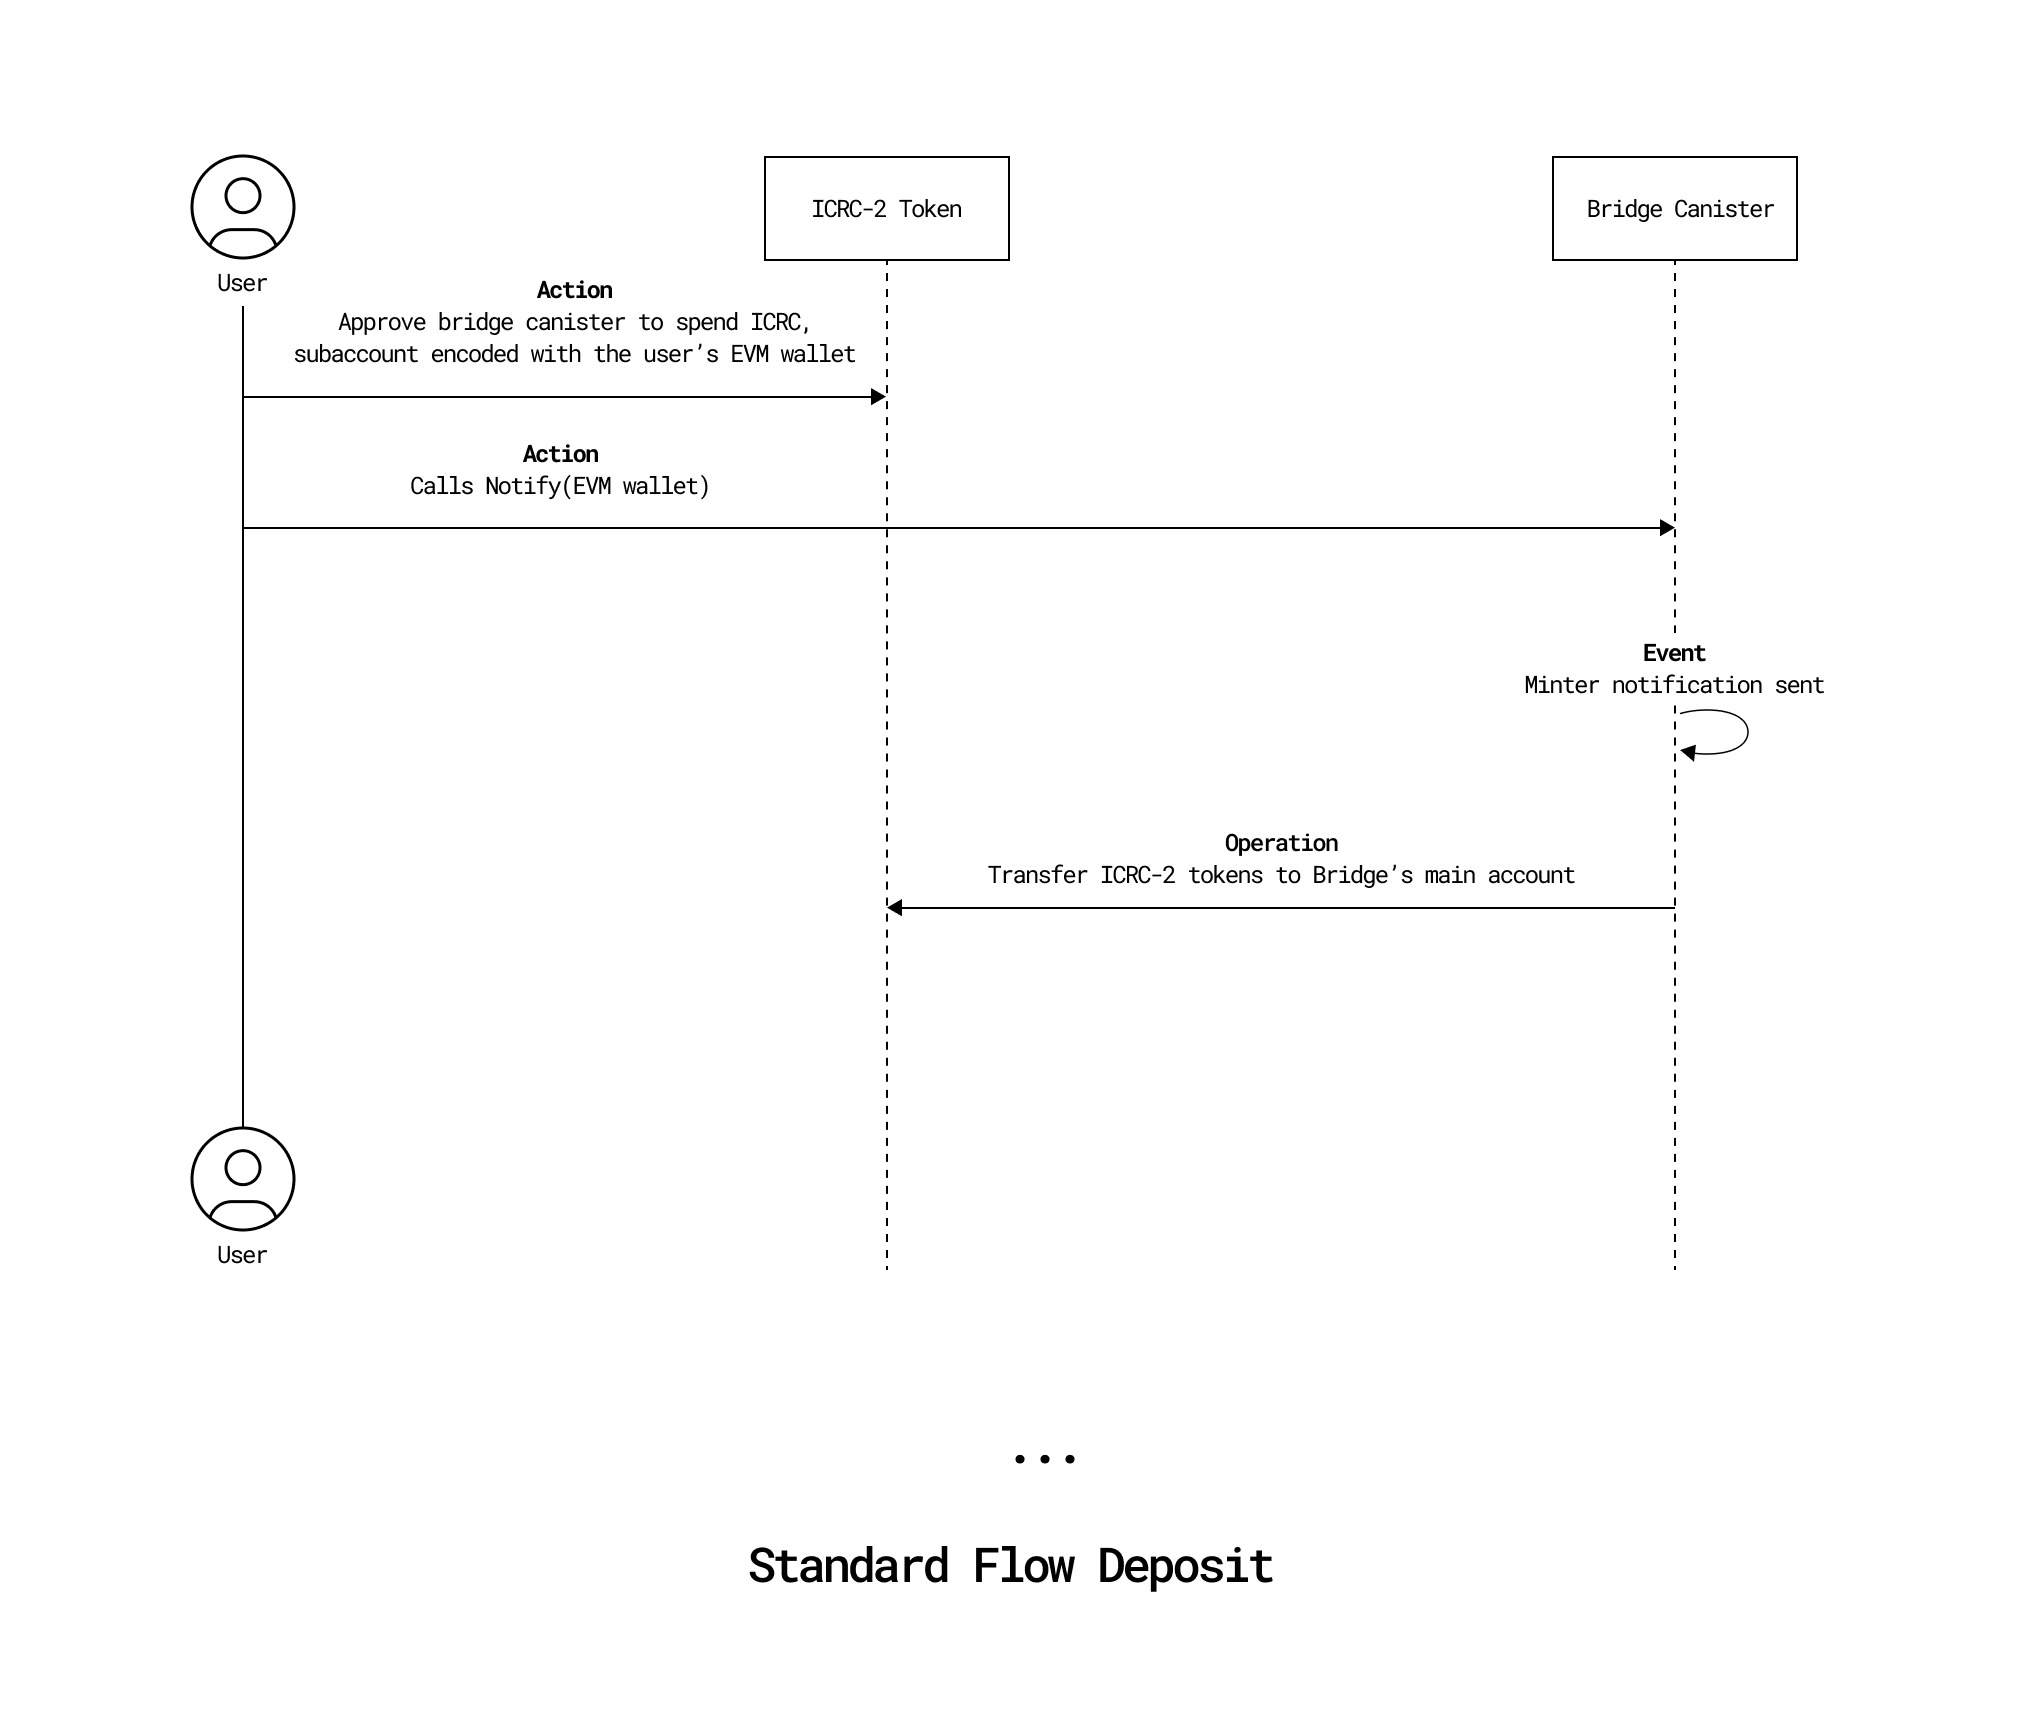
\includegraphics[width=1\textwidth]{icrc.png}
        \caption{Overview of the Deposit Flow for ICRC tokens}
        \label{fig:icrc}
    \end{figure}

After the approval of ICRC tokens, the user should call the BFT bridge notify endpoint, which triggers the onMinternotification method of the BFT bridge. 
\\
This is implemented as one step. In this step we will perform ICRC transfer from to the minter's main account. Before doing this the user should approve ICRC tokens for the special account of the ICRC bridge canister, which contains the an encoding of the Ethereum address of the recipient as a subaccount. 

\\
This is implemented as one step. In this step we will perform ICRC transfer from to the minter's main account. Before doing this the user should approve ICRC tokens for the special account of the ICRC bridge canister, which contains the an encoding of the Ethereum address of the recipient as a subaccount.


Through the use of an indexer for Runes deployed to decentralised web-servers, BitFusion offers an unparalleled level of decentralisation when Bridh



\section{Chain Abstraction: Future Directions}


\noindent Bit-Fusion does not solve the issue of providing a near-instant bridging experience from chain A to Chain B. This sort of experience can be delivered by higher level primitives, which typically involve locked

Smart-wallets via Chain-Abstraction can be used to provide a near instant bridging experience from one chain to another, which is a lower-level primitive to create secure bridges between chains via threshold signature schemes. The problem of tokens being transferred instantaneously from chain A to chain B is likely to be solved by account abstraction, threshold-signing innovations in wallet design.


\textit{An account abstraction proposal which completely avoids the need for consensus-layer protocol changes. Instead of adding new protocol features and changing the bottom-layer transaction type, this proposal introduces a higher-layer pseudo-transaction object called a UserOperation. Users send UserOperation objects into a new separate mempool. Bundlers package up a set of these objects into a single transaction by making a call to a special contract, and that transaction then gets included in a block.}

\noindent Account abstraction moves crypto from the current approach of a simple EOA account, where one can lose everything with a small mistake, to a future where an account can be tailored to their needs using smart contracts. The shift from EOAs to smart contract wallets with arbitrary verification logic paves the way for a series of improvements to wallet designs, as well as reducing complexity for end users.

\noindent The basic idea is that if you have a smart-wallet, secured by a threshold signature scheme - for instance Chain-Key, from which you could then  initiate a bridging transaction. 
Instead of directly interacting with the BitFusion bridge, a user would instead interact with a "Relay Pool". This pool would allow a relayer that has liquidity on the pool, having already bridged tokens over with BitFusion, to send the user their bridged asset with the expectation that they would receive funds from the smart-wallet. Exactly how one could do this is explained in the video here: 

https://www.youtube.com/watch?app=desktop&v=G0nFyq9DDPw&ref=blog.catalyst.exchange 

Now, we have to wait for Finality? Otherwise if the user were to get their tokens instantly on another chain, through some overcollateralised pool. 

\href{https://www.youtube.com/watch?app=desktop&v=G0nFyq9DDPw&ref=blog.catalyst.exchange}{something}